%!TEX ROOT=../diploma-thesis.tex

\chapter{Rešerše}\label{ch:reserse}

\section{Modelem ř\'{\i}zená architektura}

\todo{
\begin{itemize}
    \item Co to je MDA
    \item V\'yhody
    \item Nev\'yhody
    \item Shrnut\'{\i} a proč se nám nehod\'{\i}
\end{itemize}
}

\section{Síťové architektury}

Jak jsme již naznačili v sekci~\ref{sec:soa}, architektura orientovaná na služby staví
na počítačových síťích, díky kterým spolu mohou jednotlivé služby efektivně komunikovat.
Proto je vhodné provést rešerši základních síťových architektur,
abychom mohli co nejlépe navrhnout framework pro centrální správu
a automatickou distribuci byznysových pravidel.

\subsection{Architektura klient-server}\label{sec:client-server}

Model klient-server popisuje vztah mezi komponentami systému, klienty a serverem.
Klient zašle požadavek serveru a ten mu vrátí odpověď~\cite{berson1992client}.
Tento model může být použit obecně i v rámci jednoho počítače,
nejčastěji je však využíván v síťové komunikaci mezi více počítači.
V tomto případě klient sestaví síťové spojení k serveru a po získání odpovědi
od serveru spojení zase uzavře. Schéma komunikace je znázorněno
na obrázku ~\ref{fig:client-server}.

\begin{figure}[t]
    \centering
    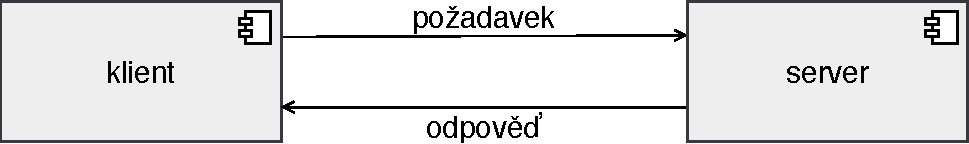
\includegraphics[keepaspectratio=true, width=0.6\linewidth]{figures/client-server.pdf}
    \caption{Architektura klient-server}
    \label{fig:client-server}
\end{figure}

Tato architektura je jednou ze základních stavebních kamenů
internetových protokolů. Je využívána zejména protokolem
\gls{TCP}~\cite{postel1981transmission}, který je využíván ke
komunikaci v síti Internet. Jako příklad si můžeme představit
prohlížení internetových stránek. Uživatel zadá \gls{URL} adresu
stránky, kterou chce navštívit, a internetový prohlížeč, potažmo uživatelův osobní počítač,
v roli klienta odešle požadavek na server nacházející se na dané adrese.
Server požadavek přijme, zpracuje, a odešle odpověď obsahující
tělo webové stránky. Klient stránku přijme a zobrazí pro koncového
uživatele.

Tento přístup má několik zásadních výhod, díky kterým se stal
široce využívaným. Díky svojí velmi obecné myšlence je nezávislý
na jakékoliv platformě a jako klient i server mohou sloužit
jak vysoce výkonné počítače, tak i osobní počítače nebo chytré telefony,
z nichž každý může využívat odlišné operační systémy –
stačí aby klient i server uměl komunikovat stejným protokolem.
Zároveň tato architektura přesouvá byznysovou logiku a
ukládání dat na server a díky tomu umožňuje
snadnější kontrolu nad systémem a jeho centrální administraci. S tím
je spojena i snažší škálovatelnost systému. V neposlední řadě
přináší model klient-server díky centralizaci i lepší zabezpečení,
kdy server může jasně definovat a vynucovat přístupová pravidla.

Hlavní nevýhodu této architektury je vytvoření jednoho centrálního bodu,
jehož výpadek ochromí funkci celého systému (v angličtině
\textit{single point of failure}). Tímto bodem je server.
Pokud na serveru nastane chyba či výpadek, žádný z klientů není schopen využívat
jeho služeb.

\subsection{Architektura Peer-to-peer}\label{sec:p2p}

Opakem modelu klient-server je síťová architektura zvaná \textit{Peer-to-peer (\gls{P2P})}.
Jednotlivé počítače v síti spolu komunikují přímo, bez centrální autority.
Všechny počítače v síti jsou si vzájemně rovnocenné.~\cite{fox2001peer}
Na obrázku~\ref{fig:peer-to-peer} je architektura znázorněna.
Hlavním cílem \gls{P2P} sítí je distribuce dat nebo výpočetních operací.

\begin{figure}[t]
    \centering
    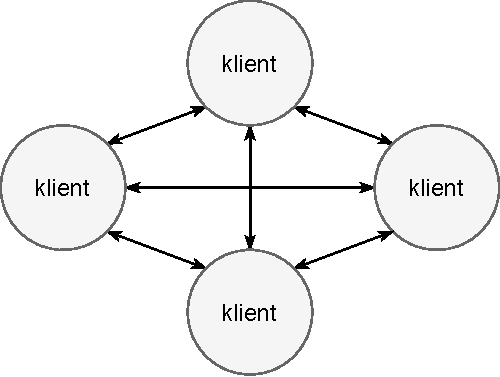
\includegraphics[keepaspectratio=true, width=0.4\linewidth]{figures/peer-to-peer.pdf}
    \caption{Architektura peer-to-peer}
    \label{fig:peer-to-peer}
\end{figure}

Jednotliví klienti mezi sebou zpravidla vytvářejí virtuální síť, tzv. \textit{overlay},
která je postavená nad fyzickou sítí, přes kterou jsou reálně zasílány zprávy.
Typicky je tato virtuální síť podmnožinou fyzické sítě. Výhodou tohoto přístupu je,
že klienti jsou abstrahováni od fyzického uspořádání počítačů a mohou spolu komunikovat napřímo,
i když mezi nimi mohou fyzicky být v síti zapojeny jiné počítače.

Nespornou výhodou architektury \gls{P2P} je, že s rostoucím počtem klientů roste i
kapacita a výkon sítě, narozdíl od modelu klient-server, kdy se klienti musí dělit o výkon serveru.
Navíc v takové síti neexistuje \textit{single point of failure} a tak se zvyšuje její robustnost.

Mezi silné nevýhody této architektury patří zvýšená bezpečnostní rizika způsobená tím,
že klienti jsou otevřeni komunikaci s jakýmkoliv jiným, potenciálně nebezpečným, klientem.
Potenciální útočník tak může velmi snadno využít zranitelností na dálku.
Další hrozbou je to, že některý z klientů může \textit{otrávit} síť podvrženými daty.
Další nevýhodou může být absence jakékoliv centrální správy sdílených dat.

\subsection{Representational state transfer}\label{sec:rest}

Representational state transfer~\cite{fielding2000rest} (\gls{REST}) je architektura
webových služeb, která staví na protokolu \gls{HTTP}, a klade na systém
několik architektonických omezení, díky kterým může systém dosáhnout
lepšího výkonu, vyšší škálovatelnosti, jednoduchému používání díky jednotnému rozhraní
a lepší odolnosti vůči chybám. V roce 2000 ho ve své dizertační práci představil Roy Fielding,
který je zároveň hlavním autorem specifikace \gls{HTTP} 1.1~\cite{fielding1999hypertext}.

\gls{REST} chápe data systému jako množinu zdrojů (z anglického \textit{resources}),
nad kterými jsou prováděny operace pomocí \gls{HTTP} požadavků. K odlišení operací
nad jedním zdrojem jsou využívány slovesa protokolu \gls{HTTP}, zejména pak \code{GET} pro čtení,
\code{POST} pro vytváření, \code{PUT} pro úpravu a \code{DELETE} pro mazání. Tím jsou zastřešeny
všechny \gls{CRUD} operace.

Principy architektury \gls{REST} jsou:

\begin{description}
    \item [Architektura klient-server] Systém by měl využívat model klient-server. Díky tomu může jasně rozdělit
    zodpovědnost za uživatelské rozhraní na klienta a zodpovědnost za ukládání dat na server. Díky tomu se zvyšuje
    škálovatelnost systému díky nižším nárokům na server.
    \item [Bezstavovost] Každý požadavek na server by měl obsahovat všechny informace potřebné k jeho vykonání.
    Kromě těla \gls{HTTP} požadavku se často využívají i hlavičky, například pro autentizaci uživatele pro
    přístup k zabezpečeným zdrojům.
    \item [Kešování] Odpovědi serveru musí obsahovat explicitní informaci o tom, zda lze odpověď uložit do cache.
    Díky tomu lze znovupoužívat data, která již server jednou vrátil, a jejich životnost má dlouhodobější charakter.
    Tím se zvyšuje výkon celého systému.
    \item [Vrstvený systém] Klient by neměl mít možnost rozeznat, zda komunikuje přímo se serverem, nebo s prostředníkem,
    např. s proxy serverem, load balancerem nebo cache.
    \item [Code-on-demand] Volitelným požadavkem na systém je tzv. \textit{code-on-demand}, který umožňuje serveru vracet
    spustitelný kód jako odpověď. Klient kód poté spustí na své straně. Typickým příkladem jsou klientské JavaScriptové aplikace spouštěné ve webových prohlížečích.
    \item [Jednotné rozhraní] Zdroje systému musejí mít unikátní identifikátor, např. \gls{URI}. Zdroje jsou při komunikaci reprezentovány libovolným formátem, který
    se může lišit od interní reprezentace zdroje v programu, např. \gls{JSON} či \gls{XML}. Reprezentace zdroje musí být
    dostatečná k tomu, aby šlo na zdroji provést úpravu či smazání. Zprávy mezi klientem a serverem musejí obsahovat veškerá potřebná metadata,
    aby druhá strana mohla zprávu plně zpracovat. K tomu se používají například \gls{HTTP} hlavičky \code{Content-type}
    či \code{Accept}, ve kterých je popsán typ reprezentace zdroje.
    Rozhraní by také mělo dodržovat koncept \textit{Hypermedia as the engine ot application state (\gls{HATEOAS})},
    který vyžaduje, aby server v odpovědích vracel metainformace o struktuře jeho \gls{API}.
    Klient je tak schopen dynamicky navigovat v rozhraní serveru aniž by bylo vyžadováno předem znát přesné adresy zdrojů.
    Princip \gls{HATEOAS} se však ve většině reálných \gls{API} zanedbává či implementuje pouze částečně
\end{description}

Nevýhody architektury \gls{REST} spočívají zejména v náročnosti její korektní implementace,
která se v praxi často zjednodušuje a tím degraduje její výhody. Přes rošířenost a popularitu
této architektury ji stále mnoho vývojářů nezná do detailu a zanedbávají některé její části.
Většina programovacích jazyků je založena na volání funkcí či metod, což svádí vývojáře ke
špatnému návrhu systému. \gls{REST} totiž naopak vyžaduje od vývojáře nad systémem přemýšlet jako
nad množinou zdrojů.

\subsection{Remote procedure call}\label{sec:rpc}

Remote procedure call (\gls{RPC}) je podstatně starší architekturou než \gls{REST}.
Tento termín byl použit již v roce 1981 Brucem Nelsonem~\cite{nelson1981remote}.
Architektura staví na modelu klient-server a její princip je velmi jednoduchý \textendash
umožňuje jednomu procesu, klientovi, zavolat proceduru na druhém, vzdáleném procesu, tedy serveru.
Klient zašle serveru zprávu, která vyžádá zavolání specifické procedury. Server
proceduru provede a po jejím dokončení zašle klientovi odpověď s návratovou hodnotou.
Klient poté může pokračovat ve své práci.

Zásadním bodem je fakt, že \gls{RPC} kompletně obstarává komunikaci, a v programu samotném
je vzdálená procedura volána stejným způsobem jako lokální procedury. Základním
prvkem architektury na klientovi i na serveru je tzv. \textit{stub}, tedy komponenta, která
umožňuje volat vzdálenou proceduru lokálně a zapozdřuje veškerou síťovou komunikaci
a serializaci či deserializaci argumentů, resp. návratových hodnot.

Představitelem architektury \gls{RPC} je například technologie \gls{CORBA},
kterou jsme již popsali v sekci~\ref{sec:corba}, nebo technologie Remote Method Invocation (\gls{RMI})
v jazyce Java. Modernějším pojetím je technologie gRPC~\cite{grpcio}
od společnosti Google\footnote{https://www.google.com/},
která je v dnešní době hojně využívána úspěšnými technologickými společnostmi.

Již zmiňovanou nevýhodou abstrakce lokálních a vzdálených volání jsou
negativní vlastnosti síťové komunikace, tedy její zvýšená latence
a nižší robustnost. Pokud programátor nemá možnost zjistit, zda volá
lokální či vzdálenou proceduru, výsledný kód může být těžké optimalizovat
a správně ošetřit výjimky, které mohou při jeho běhu nastat.

Na druhou stranu, narozdíl od \gls{REST} není pro \gls{RPC} potřeba
implementovat komplexní middleware obstarávající síťovou komunikaci,
serializaci a zpracování chyb. Middleware je zpravidla dodáván v podobě knihoven
dané technologie. Některé systémy a jejich případy použití mohou být snadněji
realizovány jako volání procedury než jako entita reprezentující systémový zdroj.

\section{Aspektově orientované programován\'{\i}}

\goal{Co je paradigma}
Programován\'{\i} je komplexn\'{\i} discipl\'{\i}na s teoreticky
neomezen\'ym počtem možnost\'{\i}, jak\'ym programátor může
řešit zadan\'y problém. Ačkoliv každá úloha má své specifické
požadavky, za relativně krátkou historii programován\'{\i} se
stihlo ustálit několik ideologi\'{\i}, tzv. programovac\'{\i}ch
paradigmat, které programátorovi poskytuj\'{\i} sadu abstrakc\'{\i}
a základn\'{\i}ch principů~\cite{van2009programming}.
D\'{\i}ky znalosti paradigmatu může programátor nejen zlepšit
svou produktivitu, ale zároveň může snáze pochopit myšlenky
jiného programátora a t\'{\i}m zlepšit kvalitu t\'ymové spolupráce.

\goal{OOP a jeho popis}
Jedn\'{\i}m z nejpopulárnějš\'{\i}ch paradigmat použ\'{\i}van\'ych k
v\'yvoji modern\'{\i}ch enterprise systémů je nepochybně
objektově orientované programován\'{\i} (\gls{OOP}). To vn\'{\i}má dan\'y problém
jako množinu objektu, které spolu intereaguj\'{\i}. Program
člen\'{\i} na malé funkčn\'{\i} celky odpov\'{\i}daj\'{\i}c\'{\i} struktuře
reálného světa~\cite{rentsch1982object}. Je vhodné zm\'{\i}nit,
že objekty se rozum\'{\i} jak konkrétn\'{\i} koncepty, např\'{\i}klad
auto nebo člověk, tak i abstraktn\'{\i} koncepty,
namátkou bankovn\'{\i} transakce nebo objednávka v obchodě.
Objekty se pak prom\'{\i}taj\'{\i} do kódu programu i do
reprezentace struktur v paměti poč\'{\i}tače.
Tento př\'{\i}stup je velmi snadn\'y pro pochopen\'{\i},
vede k lepš\'{\i}mu návrhu a organizaci programu a snižuje
tak náklady na jeho v\'yvoj a údržbu.

\goal{Nedostatky OOP}
Ačkoliv je \gls{OOP} velmi siln\'ym a všestran\'ym nástrojem,
existuj\'{\i} problémy, které nelze jeho pomoc\'{\i} efektivně řešit.
Jedn\'{\i}m takov\'ym problémem jsou obecné požadavky na systém,
které musej\'{\i} b\'yt konzistentně dodržovány na v\'{\i}ce m\'{\i}stech,
které spolu zdánlivě nesouvis\'{\i}. Př\'{\i}kladem
může b\'yt logován\'{\i} systémov\'ych akc\'{\i}, optimalizace správy paměti
nebo uniformn\'{\i} zpracován\'{\i} v\'yjimek~\cite{kiczales1997aspect}.
Takové požadavky naz\'yváme \textit{průřezové problémy}
(z anglického \textit{cross-cutting concerns}).
V rámci \gls{OOP} je programátor nucen v ojektech manuálně opakovat
kód, kter\'y zodpov\'{\i}dá za jejich realizaci. Duplikace kódu
vede k větš\'{\i} náchylnosti na lidskou chybu a k vyšš\'{\i}m nárokům na v\'yvoj
a údržbu daného softwarového systému~\cite{fowler1999refactoring}.

\goal{AOP jako odpověď na nedostatky OOP}
Aspektově orientované programován\'{\i} (\gls{AOP}) přináš\'{\i} řešen\'{\i} na
v\'yše zmiňované problémy. Extrahuje obecné požadavky,
tzv. \textit{aspekty} do jednoho m\'{\i}sta a pomoc\'{\i} procesu zvaného
\textit{weaving} je poté automaticky distribuuje do systému.
Weaving může proběhnout staticky při kompilaci programu nebo dynamicky
při jeho běhu. V obou př\'{\i}padech ale programátorovi ulehčuje práci,
protože k definici i změně aspektu docház\'{\i} centrálně a t\'{\i}m je eliminována
potřeba manuáln\'{\i} duplikace kódu. Je nutno poznamenat, že \gls{AOP} nen\'{\i}
paradigmatem poskytuj\'{\i}c\'{\i}m kompletn\'{\i} framework pro návrh programu.
V ideáln\'{\i}m př\'{\i}padě je tedy k návrhu systému využita kombinace
\gls{AOP} s jin\'ym paradigmatem. Pro účely této práce se zaměř\'{\i}me na
kombinaci \gls{AOP} a \gls{OOP}.

\todo{
\begin{itemize}
    \item diagram cross cutting concerns
    \item roztáhnout do v\'{\i}ce odstavců
    \item diagram weaveru
    \item section BPEL
\end{itemize}
}

\begin{description}
    \item [Aspekt]
    \item [Join-point]
    \item [Pointcut]
    \item [Advice]
    \item [Weaving]
\end{description}

\section{Aspect-driven Design Approach}

\todo{
\begin{itemize}
    \item co to je
    \item jak nám to pomůže
    \item využ\'{\i}t\'{\i} jeho konceptů
    \item shrnut\'{\i}
\end{itemize}
}

Aspect-driven Design Approach (\gls{ADDA})

\goal{Vhodnost AOP pro náš úkol}
Vzhledem k požadavkům na implementaci našeho frameworku stanoven\'ym
v předchoz\'{\i} kapitole~\ref{ch:analyza} se \gls{AOP} a na něm stavěj\'{\i}c\'{\i} \gls{ADDA}
jev\'{\i} jako vhodn\'y př\'{\i}stup, kter\'y nám pomůže dosáhnout c\'{\i}le.

\section{Stávaj\'{\i}c\'{\i} řešen\'{\i} reprezentace business pravidel}

\subsection{Drools DSL}

\todo{
\begin{itemize}
    \item co to je
    \item jak to funguje
    \item RETE algoritmus
    \item v\'yhody
    \item nev\'yhody
    \item shrnut\'{\i} a proč se nám nehod\'{\i}
\end{itemize}
}

\goal{Drools se nám nehod\'{\i}, protože je jen pro platformu Java}
...

\subsection{JetBrains MPS}

\todo{
\begin{itemize}
    \item co to je
    \item jak to funguje
    \item v\'yhody
    \item nev\'yhody
    \item shrnut\'{\i} a proč se nám nehod\'{\i}
\end{itemize}
}

\goal{MPS je super, ale nevyhovuje nám kvůli dynamick\'ym změnám}
...

\section{Shrnut\'{\i}}

V této kapitole jsme provedli rešerši \textit{modelem řízené architektury},
jej\'{\i}ch v\'yhod a nev\'yhod. Dále jsme prozkoumali, jak\'y způsobem funguje
s\'{\i}ťová \textit{architektura klient-server}, jaké jsou v\'yhody a nev\'yhody
a shrnuli jsme paradigma \textit{aspektově orientovaného programován\'{\i}} a
z něch vycházej\'{\i}c\'{\i} př\'{\i}stup k návrhu softwarov\'ych systémů \textit{ADDA}.
Nakonec jsme provedli rešerši stávaj\'{\i}c\'{\i}ch řešen\'{\i} reprezentace byznys pravidel
včetně komplexn\'{\i}ho frameworku \textit{Drools} a zhodnotili jsme jeho vhodnost
k řešen\'{\i} našeho problému. % TODO: revize podle toho co tu opravdu bude
